\chapter{Mensajeros químicos y transducción de señales}\label{ch:b2:cell-signalling}

Una sola molécula de adrenalina que llega a la superficie de una célula
hepática nunca entra en ella. Se une a una proteína del exterior, cambia
la forma de esa proteína y, en un segundo, la célula ha fabricado diez
mil moléculas de un \omterm{prop:b2:cell-signalling:gpcr}{segundo mensajero}, ha activado cien mil moléculas de
enzima y ha empezado a liberar un millón de moléculas de glucosa --- una
cadena de amplificaciones de un factor de un millón, iniciada por una
señal que se quedó al otro lado de la puerta. Este capítulo trata de los
mensajeros que las células se envían unas a otras y de cómo una célula
convierte un mensaje recibido en su superficie en un cambio de su
química, de sus genes o de su forma: los receptores, los \omterm{prop:b2:cell-signalling:gpcr}{segundos
mensajeros}, las cascadas de quinasas y los dos diseños --- la señalización
rápida y cableada de los nervios y la señalización lenta y difundida de
las \omterm{def:b2:cell-signalling:kinds}{hormonas} --- cuyo contraste recorre el resto de este libro.

\section{Los mensajeros}

\begin{definition}[Tipos de señalización química]\label{def:b2:cell-signalling:kinds}
\index{hormona}\index{señalización endocrina}\index{señalización paracrina}\index{neurotransmisor}
Una célula envía una señal a otra mediante una molécula secretada, un
\emph{mensajero} o \emph{ligando}, que se une a un \emph{receptor} situado
en la superficie o en el interior de la célula diana. Según el alcance: la
señalización \emph{endocrina}, en la que una glándula libera una
\emph{hormona} a la \omterm{def:b2:blood-circulation:blood}{sangre}, que llega a todas las células del cuerpo y
solo actúa sobre las que poseen el receptor, en un plazo de minutos a
horas (insulina, cortisol, adrenalina, tiroxina); la señalización
\emph{paracrina}, en la que el mensajero difunde hacia células vecinas
situadas a menos de un milímetro y se destruye por el camino (factores
de crecimiento, histamina, prostaglandinas, los morfógenos del
\cref{ch:b2:vertebrate-development}); la \emph{autocrina}, en la que la
célula se envía la señal a sí misma; y la \emph{sináptica}, en la que una
neurona libera un \emph{neurotransmisor} a través de un espacio de
\qty{20}{nm} sobre una sola célula diana, en un milisegundo
(\cref{ch:b2:neurons-synapses}).
Según su química: los mensajeros \emph{hidrosolubles} --- derivados de
aminoácidos como la adrenalina, péptidos y proteínas como la
insulina --- no pueden atravesar la membrana y actúan sobre receptores de
superficie; los mensajeros \emph{liposolubles} --- los esteroides
(cortisol, estradiol, testosterona), la tiroxina, el ácido retinoico, el
óxido nítrico --- la atraviesan y actúan sobre receptores internos. Los
sistemas endocrino y nervioso son las dos maneras en que un cuerpo de
$10^{13}$ células se coordina: uno difunde despacio a todos, el otro
conecta deprisa con alguien concreto.
\end{definition}
\begin{omfigure}
\begin{tikzpicture}[every node/.style={font=\scriptsize}, >=stealth]
  % endocrine
  \begin{scope}
    \draw[thick, fill=omProp!25] (0,1.6) circle (0.35); \node[above] at (0,2.0) {glándula};
    \draw[very thick, omThm!60] (-0.5,0.6) -- (4.5,0.6); \draw[very thick, omThm!60] (-0.5,0.2) -- (4.5,0.2); \node[omThm!70!black] at (2,0.4) {sangre};
    \foreach \x in {0.6,1.5,2.4,3.3} \fill[omProp] (\x,0.4) circle (0.05);
    \draw[->, omProp] (0,1.25) -- (0,0.65);
    \draw[thick, fill=omDef!20] (3.8,-0.8) circle (0.35); \node[below, align=center] at (3.8,-1.2) {célula diana\\con receptor};
    \draw[->, omProp] (3.8,0.15) -- (3.8,-0.4);
    \draw[thick, fill=gray!20] (1.0,-0.8) circle (0.35); \node[below, align=center] at (1.0,-1.2) {sin receptor:\\la ignora};
    \node[align=center] at (2.2,-2.4) {endocrina: hormona en la sangre,\\todo el cuerpo, de minutos a horas};
  \end{scope}
  % paracrine
  \begin{scope}[xshift=6.6cm]
    \draw[thick, fill=omProp!25] (0.8,0.6) circle (0.35);
    \foreach \a in {0,45,...,315} \fill[omProp] (0.8,0.6) ++(\a:0.6) circle (0.04);
    \draw[thick, fill=omDef!20] (1.9,0.9) circle (0.3); \draw[thick, fill=omDef!20] (1.7,-0.2) circle (0.3); \draw[thick, fill=omDef!20] (-0.2,0.0) circle (0.3);
    \node[align=center] at (0.8,-2.4) {paracrina: difunde a\\las vecinas, destruida\\en un milímetro};
  \end{scope}
  % synaptic
  \begin{scope}[xshift=11.6cm]
    \draw[very thick, omDef] (0,1.8) -- (0,0.5); \draw[thick, fill=omDef!25] (0,0.3) circle (0.25);
    \draw[thick, fill=omExo!30] (0,-0.5) circle (0.3);
    \foreach \x in {-0.08,0,0.08} \fill[omProp] (\x,-0.05) circle (0.03);
    \node[align=center] at (0.2,-2.4) {sináptica: una diana,\\\qty{20}{nm},\\un milisegundo};
  \end{scope}
\end{tikzpicture}

{\small Tres alcances de la señalización química: una \omterm{def:b2:cell-signalling:kinds}{hormona} difundida
por la \omterm{def:b2:blood-circulation:blood}{sangre} a todas las células que portan su receptor; un factor
paracrino que llega a sus vecinas; un \omterm{def:b2:cell-signalling:kinds}{neurotransmisor} entregado a una
sola célula a través de una sinapsis.}
\end{omfigure}

\begin{theorem}[Ocupación de los receptores]\label{thm:b2:cell-signalling:occupancy}
\index{constante de disociación}\index{ocupación de los receptores}
Un receptor $R$ se une a su ligando $L$ de forma reversible, $R + L
\rightleftharpoons RL$, con una \emph{\omterm{thm:b2:cell-signalling:occupancy}{constante de disociación}} $K_d =
[R][L]/[RL]$. En el equilibrio, la fracción de receptores ocupados es
\[
\theta = \frac{[RL]}{[R]_{\text{tot}}} = \frac{[L]}{K_d + [L]},
\]
la misma hipérbola que la saturación de una enzima. $K_d$ es la
concentración a la que la mitad de los receptores están ocupados y mide
la \emph{afinidad}: cuanto menor, más fuerte la unión. Los receptores
hormonales tienen una $K_d$ del orden nanomolar a picomolar, ajustada a
las concentraciones a las que circulan las \omterm{def:b2:cell-signalling:kinds}{hormonas} ($10^{-12}$ a
$10^{-9}$ mol/L): a $[L] = K_d/10$ está ocupada una décima parte, a
$10K_d$ nueve décimas. Una célula no puede responder a una \omterm{def:b2:cell-signalling:kinds}{hormona} para la
que no tiene receptores, y ajusta su sensibilidad cambiando el número de
receptores o --- como en el \cref{ch:b2:reproductive-hormones} ---
retirándolos cuando la \omterm{def:b2:cell-signalling:kinds}{hormona} está presente de forma constante.
\end{theorem}
\begin{proof}
Con $[R] = [R]_{\text{tot}} - [RL]$, $K_d = ([R]_{\text{tot}} -
[RL])[L]/[RL]$, de modo que $[RL](K_d + [L]) = [R]_{\text{tot}}[L]$, que es
la fórmula. Es la expresión de Michaelis--Menten del volumen del primer
año sin la etapa catalítica.
\end{proof}

\begin{omfigure}
\begin{tikzpicture}
\begin{axis}[
  width=0.68\linewidth, height=5.2cm,
  axis x line=bottom, axis y line=left,
  xmode=log, xmin=0.01, xmax=100, ymin=0, ymax=1.1,
  xlabel={concentración de ligando (en unidades de $K_d$)}, ylabel={fracción de receptores ocupados},
  xlabel style={font=\small, at={(axis description cs:0.5,-0.13)}, anchor=north},
  ylabel style={font=\small},
  tick label style={font=\small}, xtick={0.01,0.1,1,10,100}, ytick={0,0.5,1},
  clip=false,
]
\addplot[very thick, omDef, domain=0.01:100, samples=100] {x/(1+x)};
\draw[dashed, gray] (axis cs:1,0) -- (axis cs:1,0.5) -- (axis cs:0.01,0.5);
\node[font=\scriptsize, anchor=north west] at (axis cs:1.1,0.48) {$[L] = K_d$: la mitad ocupados};
\node[font=\scriptsize, anchor=south east] at (axis cs:0.1,0.1) {10\% at $K_d/10$};
\node[font=\scriptsize, anchor=north west] at (axis cs:10,0.92) {90\% at $10\,K_d$};
\end{axis}
\end{tikzpicture}

{\small \omterm{thm:b2:cell-signalling:occupancy}{Ocupación de los receptores} frente a la concentración de ligando
en escala logarítmica: la respuesta de una célula pasa de una décima a
nueve décimas en un intervalo de concentraciones de un factor cien
centrado en $K_d$.}
\end{omfigure}

\section{Receptores de superficie}

\begin{proposition}[Receptores acoplados a proteínas G y AMP cíclico]\label{prop:b2:cell-signalling:gpcr}
\index{proteína G}\index{receptor acoplado a proteínas G}\index{AMP cíclico}\index{segundo mensajero}\index{proteína quinasa A}
La familia de receptores más numerosa --- unos \num{800} genes en el ser
humano, para \omterm{def:b2:cell-signalling:kinds}{hormonas}, \omterm{def:b2:cell-signalling:kinds}{neurotransmisores}, olores, luz --- está formada por
proteínas que atraviesan la membrana siete veces. Un ligando que se une en
el exterior cambia su conformación en el interior, donde el receptor
activa una \emph{\omterm{prop:b2:cell-signalling:gpcr}{proteína G}}: un interruptor de tres subunidades que cambia el GDP
unido por GTP, se separa y, en su forma unida al GTP, regula una enzima
efectora durante unos segundos antes de hidrolizar el GTP y apagarse. El
efector clásico es la \emph{adenilato ciclasa}, que fabrica \emph{\omterm{prop:b2:cell-signalling:gpcr}{AMP
cíclico}} a partir de ATP: un \emph{\omterm{prop:b2:cell-signalling:gpcr}{segundo mensajero}} pequeño y difusible
cuya concentración sube en segundos de \qty{0.1}{\micro mol/L} a varios
micromolar y que activa la \emph{\omterm{prop:b2:cell-signalling:gpcr}{proteína quinasa A}}, una enzima que
fosforila --- y así activa o desactiva --- decenas de proteínas diana. La
señal termina gracias a la fosfodiesterasa, que destruye el AMPc, y a las
fosfatasas, que retiran los fosfatos. La adrenalina actúa así sobre una
célula hepática: receptor $\to$ \omterm{prop:b2:cell-signalling:gpcr}{proteína G}
$\to$ ciclasa $\to$ AMPc $\to$ quinasa A $\to$ fosforilasa quinasa
$\to$ glucógeno fosforilasa $\to$ glucosa. El glucagón sigue la misma
vía; otras \omterm{prop:b2:cell-signalling:gpcr}{proteínas G} inhiben la ciclasa, o activan la fosfolipasa C,
que libera otros dos \omterm{prop:b2:cell-signalling:gpcr}{segundos mensajeros}, el \emph{inositol trifosfato}
--- que abre los depósitos de calcio --- y el diacilglicerol.
\end{proposition}
\begin{proof}[Evidencia]
Sutherland (1957) demostró que la adrenalina añadida a un homogeneizado
de hígado solo liberaba glucosa si había membranas, que las membranas
producían un factor termoestable que activaba por sí solo la fosforilasa
en la fracción sin membranas, y que ese factor era el \omterm{prop:b2:cell-signalling:gpcr}{AMP cíclico} --- el
primer \omterm{prop:b2:cell-signalling:gpcr}{segundo mensajero}, y la primera demostración de que una \omterm{def:b2:cell-signalling:kinds}{hormona}
actúa en la superficie celular a través de un intermediario intracelular.
Rodbell y Gilman (década de 1970) descubrieron que la ciclasa necesitaba
GTP y aislaron la \omterm{prop:b2:cell-signalling:gpcr}{proteína G} que transmite la señal entre el receptor y
la enzima; la toxina colérica, que bloquea la \omterm{prop:b2:cell-signalling:gpcr}{proteína G} en su estado
activo, hace que el intestino secrete litros de líquido al día --- la
enfermedad es un defecto de la señalización.
\end{proof}

\begin{omfigure}
\begin{tikzpicture}[every node/.style={font=\scriptsize}, >=stealth]
  % membrane
  \fill[omExo!30] (0,2.0) rectangle (12,2.5);
  \node[anchor=east] at (-0.1,2.25) {membrana};
  % receptor
  \draw[thick, fill=omDef!40] (1.0,1.7) rectangle (1.8,2.8); \node[anchor=east] at (0.95,2.65) {receptor};
  \fill[omProp] (1.4,3.35) circle (0.12); \node[omProp, above] at (1.4,3.45) {adrenalina};
  \draw[->, omProp] (1.4,3.23) -- (1.4,2.85);
  % G protein
  \draw[thick, fill=omDef!25] (2.6,1.5) ellipse (0.72 and 0.36); \node at (2.6,1.5) {proteína G};
  \node[below] at (2.6,1.1) {GDP $\to$ GTP};
  \draw[->, thick] (1.8,2.0) -- (2.2,1.75);
  % cyclase
  \draw[thick, fill=omDef!40] (4.2,1.7) rectangle (5.2,2.8); \node[above] at (4.7,2.85) {adenilato ciclasa};
  \draw[->, thick] (3.15,1.5) -- (4.2,1.85);
  % cAMP
  \node[omThm, anchor=west] at (5.35,1.55) {ATP $\to$ AMPc};
  \draw[->, thick, omThm] (4.7,1.7) -- (5.2,1.15);
  % PKA
  \draw[thick, fill=omThm!20] (7.3,0.9) ellipse (0.7 and 0.35); \node at (7.3,0.9) {quinasa A};
  \draw[->, thick, omThm] (6.4,0.9) -- (6.6,0.9);
  % targets
  \draw[->, thick] (8.0,0.9) -- (9.0,0.9);
  \node[anchor=west, align=left] at (9.0,0.9) {fosforilasa quinasa $\to$ fosforilasa\\$\to$ glucógeno $\to$ glucosa};
  % amplification annotations
  \node[gray, align=center] at (1.4,0.3) {1 hormona};
  \node[gray, align=center] at (4.7,0.3) {$\sim 10^{2}$ proteínas G};
  \node[gray, align=center] at (7.3,0.3) {$\sim 10^{4}$ AMPc};
  \node[gray, align=center] at (10.2,0.3) {$\sim 10^{6}$ glucosa};
  % off switches
  \node[omExo!70!black, align=center, anchor=south] at (9.6,2.7) {apagado: hidrólisis del GTP (segundos),\\la fosfodiesterasa destruye el AMPc,\\las fosfatasas deshacen las fosforilaciones};
\end{tikzpicture}

{\small La vía del \omterm{prop:b2:cell-signalling:gpcr}{AMP cíclico}, de la adrenalina a la glucosa. Cada etapa
activa muchas copias de la siguiente: una sola molécula de \omterm{def:b2:cell-signalling:kinds}{hormona} acaba
en un millón de moléculas de producto.}
\end{omfigure}

\begin{theorem}[Amplificación en una cascada]\label{thm:b2:cell-signalling:amplification}
\index{amplificación (señalización)}
Si cada una de las $n$ etapas de una cascada activa $a$ moléculas de la
siguiente durante el tiempo que dura su propia activación, una molécula
de mensajero produce $a^{n}$ moléculas del producto final. Con cuatro
etapas amplificadoras de cien cada una --- un receptor que activa cien
\omterm{prop:b2:cell-signalling:gpcr}{proteínas G}, una ciclasa que fabrica cien AMPc, una quinasa que fosforila
cien enzimas, una enzima que libera cien moléculas de
glucosa --- $a^{n} = 10^{8}$; en la práctica, un millón más o menos,
en unos segundos, a partir de una \omterm{def:b2:cell-signalling:kinds}{hormona} a $10^{-9}$ mol/L. La
amplificación explica que las \omterm{def:b2:cell-signalling:kinds}{hormonas} puedan ser eficaces a
concentraciones un millón de veces inferiores a las de los metabolitos que
controlan, y que la cascada deba poder apagarse en cada etapa: un
amplificador que no se puede apagar es una enfermedad (el cólera, y los
numerosos cánceres en los que una proteína de señalización queda
bloqueada en estado activo).
\end{theorem}
\begin{proof}
La etapa 1 produce $a$ moléculas activas; cada una produce $a$
en la etapa 2, lo que da $a^{2}$; por inducción, $a^{n}$ tras $n$ etapas.
La ganancia de cada etapa es el número de ciclos catalíticos que realiza
un catalizador activado antes de inactivarse: su velocidad catalítica
por su tiempo de vida activo.
\end{proof}

\begin{proposition}[Receptores tirosina quinasa y calcio]\label{prop:b2:cell-signalling:rtk}
\index{receptor tirosina quinasa}\index{receptor de la insulina}\index{señalización por calcio}\index{calmodulina}
Una segunda familia de receptores de superficie --- los de la insulina,
los de los factores de crecimiento que impulsan la división celular, los
de las señales inductoras del desarrollo --- son los \emph{\omterm{prop:b2:cell-signalling:rtk}{receptores
tirosina quinasa}}: proteínas de un solo paso transmembrana que, cuando su
ligando reúne dos de ellas, se fosforilan mutuamente en tirosinas y crean
así sitios de anclaje para un conjunto de proteínas adaptadoras. De ellos
parten varias cascadas a la vez: una cadena de tres quinasas (la cascada
de las MAP quinasas) que termina en el núcleo y activa los genes del
crecimiento; una quinasa de lípidos cuyo producto recluta la quinasa que
media los efectos metabólicos de la insulina --- desplazar los
transportadores de glucosa a la membrana, activar la síntesis de
glucógeno ---; y otras. Un tercer \omterm{prop:b2:cell-signalling:gpcr}{segundo mensajero} universal es el
\emph{calcio}: mantenido en el citosol a \qty{0.1}{\micro mol/L}, diez mil
veces por debajo del exterior, entra en masa por canales abiertos por una
señal o por un voltaje, o sale del retículo endoplásmico en respuesta al
inositol trifosfato, y sube a concentraciones micromolares en
milisegundos; unido a la \emph{calmodulina} activa quinasas y bombas, y
unido a la troponina desencadena la contracción
(\cref{ch:b2:muscle-movement}). Las bombas lo devuelven a los depósitos
en menos de un segundo. Sea cual sea el receptor, el interior de la célula
habla unos pocos lenguajes --- AMPc, calcio, fosforilación --- y la
especificidad reside en las proteínas que cada tipo celular posee para
que esos lenguajes actúen sobre ellas.
\end{proposition}

\begin{omfigure}
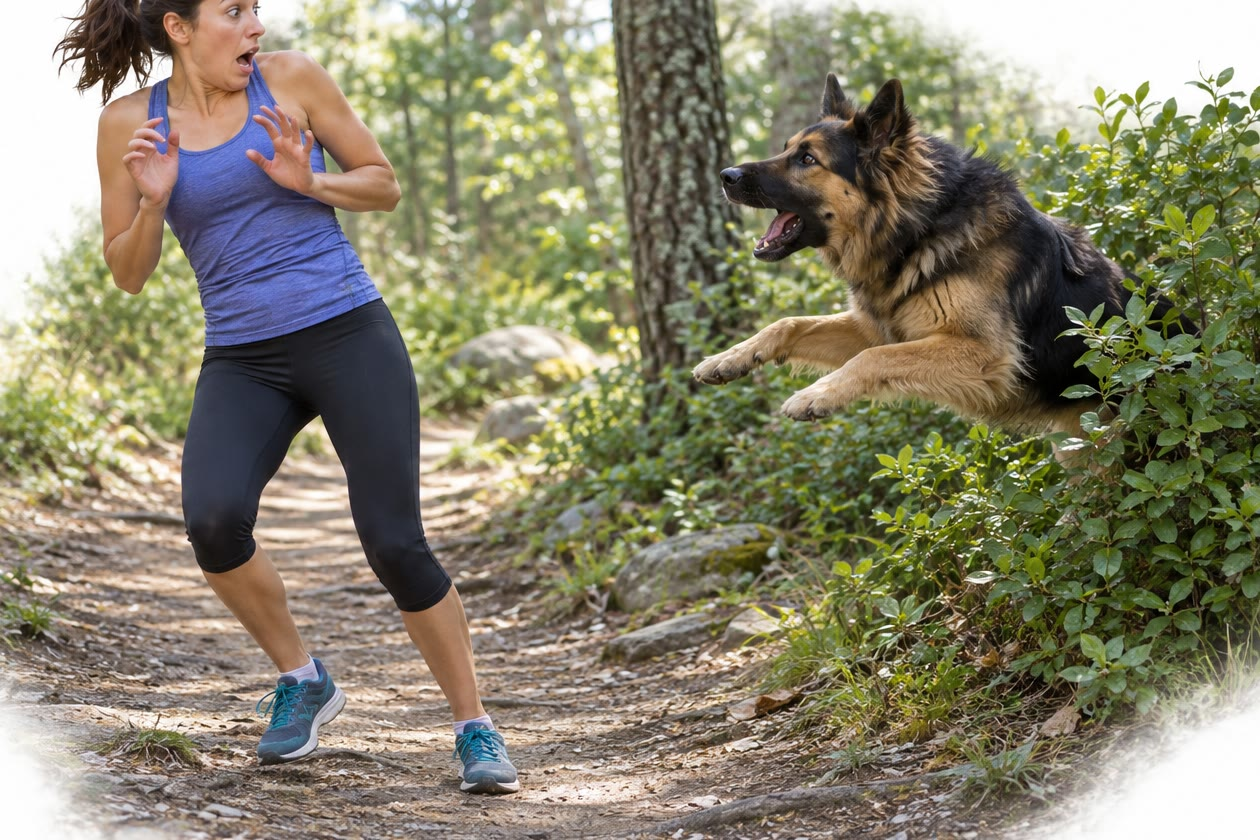
\includegraphics[width=0.6\linewidth]{images/book4/ai/b4-19-adrenaline-runner.jpg}

{\small La cascada en acción. Un susto libera adrenalina de la médula
suprarrenal; en segundos el \omterm{def:b2:heart:anatomy}{corazón} se acelera, el hígado vierte glucosa y
las vías respiratorias se ensanchan --- un mensajero, varios receptores,
una amplificación de un millón en cada célula.}
\end{omfigure}

\section{Receptores internos}

\begin{proposition}[Receptores nucleares]\label{prop:b2:cell-signalling:nuclear}
\index{receptor nuclear}\index{hormona esteroidea}
Los esteroides, la tiroxina, el ácido retinoico y la vitamina D difunden a
través de la membrana y se unen a receptores del citosol o del núcleo que
son a su vez \emph{\omterm{prop:b2:cell-differentiation:transcriptional}{factores de transcripción}}: el complejo
hormona--receptor se une a secuencias específicas de ADN y activa o
desactiva sus genes diana. La respuesta es lenta --- de minutos a horas
para fabricar el ARNm y la proteína --- y duradera: el cortisol induce las
enzimas de la gluconeogénesis durante horas, el estradiol construye el
revestimiento uterino a lo largo de días, la testosterona fabrica músculo
a lo largo de semanas, la tiroxina fija la tasa metabólica de todas las
células. Algunos esteroides tienen también acciones rápidas a través de
receptores de superficie, y algunas vías de superficie llegan también al
núcleo (la cascada de las MAP quinasas), de modo que la distinción no es
absoluta; pero la regla se mantiene: un mensajero liposoluble cambia lo
que una célula \emph{es} cambiando sus genes, mientras que uno
hidrosoluble cambia lo que \emph{hace} cambiando sus
enzimas.
\end{proposition}

\begin{omfigure}
\begin{tikzpicture}[every node/.style={font=\scriptsize}, >=stealth]
  \foreach \x/\t in {0/{hidrosolubles: adrenalina, insulina, glucagón}, 7.4/{liposolubles: cortisol, estradiol, tiroxina}} \node[anchor=south, font=\scriptsize\bfseries] at (\x+2.6,3.4) {\t};
  % left: surface receptor
  \fill[omExo!30] (0,2.4) rectangle (5.2,2.8);
  \draw[thick, fill=omDef!40] (1.6,2.1) rectangle (2.3,3.1);
  \fill[omProp] (1.95,3.35) circle (0.1);
  \draw[->, thick] (1.95,2.1) -- (1.95,1.6) node[below, align=center] {segundos mensajeros,\\quinasas: enzimas\\activadas en segundos};
  \node[align=center] at (4.5,1.0) {cambia lo que\\la célula hace};
  % right: nuclear receptor
  \begin{scope}[xshift=7.4cm]
    \fill[omExo!30] (0,2.4) rectangle (5.2,2.8);
    \fill[omProp] (1.5,3.35) circle (0.1);
    \draw[->, omProp] (1.5,3.25) -- (1.5,1.9);
    \draw[thick, fill=omThm!20] (1.5,1.5) ellipse (0.72 and 0.3); \node at (1.5,1.5) {receptor};
    \draw[thick] (0.6,0.4) -- (4.6,0.4); \draw[thick] (0.6,0.25) -- (4.6,0.25); \node[below] at (2.6,0.2) {ADN: genes diana activados o no, horas};
    \draw[->, thick] (1.5,1.2) -- (2.4,0.5);
    \node[align=center] at (4.0,1.4) {cambia lo que\\la célula es};
  \end{scope}
\end{tikzpicture}

{\small Dos diseños. Un mensajero hidrosoluble actúa en la superficie y
cambia la actividad enzimática en segundos; uno liposoluble entra, se une
a un receptor que es un \omterm{prop:b2:cell-differentiation:transcriptional}{factor de transcripción} y cambia la expresión
génica a lo largo de horas.}
\end{omfigure}

\section{Un caso práctico: la insulina, el glucagón y el valor de consigna de la glucemia}

\begin{proposition}[Dos hormonas y un valor de consigna]\label{prop:b2:cell-signalling:glucose}
\index{insulina}\index{glucagón}\index{glucemia}
La glucosa de la \omterm{def:b2:blood-circulation:blood}{sangre} se mantiene cerca de \qty{5}{mmol/L}
(\qty{0.9}{g/L}) gracias a dos \omterm{def:b2:cell-signalling:kinds}{hormonas} antagonistas de los islotes
pancreáticos. Tras una comida, la glucosa que sube es detectada por las
células $\beta$ --- que la metabolizan, cierran un canal de potasio al
subir su ATP, se despolarizan, dejan entrar calcio y liberan
\emph{insulina} --- y la insulina, a través de su \omterm{prop:b2:cell-signalling:rtk}{receptor tirosina
quinasa}, hace que el músculo y el tejido adiposo capten glucosa
(desplazando transportadores a sus membranas), que el hígado la almacene
como glucógeno y grasa, y que todos los tejidos dejen de quemar grasa.
Entre comidas, la glucosa que baja permite a las células $\alpha$ liberar
\emph{glucagón}, que, a través del AMPc en el hígado, degrada el glucógeno
y fabrica glucosa nueva a partir de aminoácidos; la adrenalina hace lo
mismo más deprisa en las urgencias, y el cortisol y la \omterm{def:b2:cell-signalling:kinds}{hormona} del
crecimiento a lo largo de horas. Cada \omterm{def:b2:cell-signalling:kinds}{hormona} se libera en proporción a la
desviación que corrige: una retroalimentación negativa con dos efectores,
uno para cada sentido, y un valor de consigna defendido con un margen de
una quinta parte. El encéfalo, que quema \qty{120}{g} de glucosa al día y
no almacena nada, es el órgano que el bucle protege; la diabetes de
tipo 1 es la pérdida de las células $\beta$, y su evolución sin
tratamiento --- glucosa a \qty{20}{mmol/L}, grasa quemada por falta de
insulina, ácido en la \omterm{def:b2:blood-circulation:blood}{sangre} --- es el aspecto del bucle cuando se le
quita un brazo.
\end{proposition}

\begin{omfigure}
\begin{tikzpicture}
\begin{axis}[
  width=0.82\linewidth, height=5.6cm,
  axis x line=bottom, axis y line=left,
  xmin=0, xmax=6, ymin=0, ymax=1.1,
  xlabel={horas después de una comida}, ylabel={relativo al máximo},
  xlabel style={font=\small, at={(axis description cs:0.5,-0.12)}, anchor=north},
  ylabel style={font=\small},
  tick label style={font=\small}, xtick={0,1,2,3,4,5,6}, ytick={0,0.5,1},
  legend style={font=\scriptsize, at={(0.5,-0.28)}, anchor=north, draw=none, legend columns=3},
  clip=false,
]
\addplot[very thick, omDef, domain=0:6, samples=80] {0.55 + 0.45*exp(-((x-0.9)^2)/0.5) - 0.08*exp(-((x-4)^2)/2)};
\addlegendentry{glucemia (5 mmol/L a 0,55)}
\addplot[very thick, omThm, domain=0:6, samples=80] {0.15 + 0.85*exp(-((x-1.1)^2)/0.45)};
\addlegendentry{insulina}
\addplot[very thick, omProp, domain=0:6, samples=80] {0.75 - 0.5*exp(-((x-1.2)^2)/0.8) + 0.25*(1-exp(-x/5))*0.6};
\addlegendentry{glucagón}
\end{axis}
\end{tikzpicture}

{\small Glucosa, insulina y glucagón tras una comida. La insulina sube con
la glucosa y la hace bajar; cuando la glucosa desciende hacia el valor de
consigna, el glucagón sube para mantenerla en él.}
\end{omfigure}

\begin{example}[Velocidad, alcance y coste de los dos sistemas]\label{ex:b2:cell-signalling:compare}
La adrenalina de la \omterm{def:b2:blood-circulation:blood}{sangre} llega a todas las células en alrededor de un
minuto (el tiempo de circulación) y actúa durante minutos; un impulso
nervioso llega a su diana en milisegundos y actúa durante milisegundos.
Una \omterm{def:b2:cell-signalling:kinds}{hormona} no cuesta casi nada por célula alcanzada --- un nanomol
repartido por el cuerpo ---, pero no puede dirigirse a una sola célula; un
nervio se dirige exactamente a una célula, pero debe construir y mantener
un cable hasta ella. El cuerpo usa ambos: los nervios simpáticos del
\cref{ch:b2:blood-pressure} actúan sobre el \omterm{def:b2:heart:anatomy}{corazón} y las \omterm{def:b2:blood-circulation:vessels}{arteriolas} en
un segundo, y la médula suprarrenal, que es en sí misma un ganglio
simpático modificado, los respalda vertiendo la misma molécula en la
\omterm{def:b2:blood-circulation:blood}{sangre} para todo el cuerpo. Y en la sinapsis los dos diseños se
encuentran, pues un \omterm{def:b2:cell-signalling:kinds}{neurotransmisor} es un mensajero que actúa sobre un
receptor mediante los mismos mecanismos --- un canal que se abre, una
\omterm{prop:b2:cell-signalling:gpcr}{proteína G} que se activa ---, solo que a través de veinte nanómetros en
lugar de un metro.
\end{example}

\section{Ejercicios}

\begin{exercise}[$\star$]\label{exo:b2:cell-signalling:1}
Clasifíquense como endocrinos, paracrinos, autocrinos o sinápticos, y como
hidrosolubles o liposolubles: la insulina, el cortisol, la acetilcolina en
una sinapsis, la histamina en una herida, el estradiol, la adrenalina de
la glándula suprarrenal, el óxido nítrico del endotelio.
\end{exercise}

\begin{exercise}[$\star$]\label{exo:b2:cell-signalling:2}
Enumérense las etapas que van de la adrenalina en la membrana de la célula
hepática a la glucosa en la \omterm{def:b2:blood-circulation:blood}{sangre}, y nómbrese el interruptor de apagado
de cada etapa.
\end{exercise}

\begin{exercise}[$\star$]\label{exo:b2:cell-signalling:3}
Compárense los receptores de superficie y los nucleares: qué se une a
ellos, dónde están, con qué rapidez actúan y qué cambian.
\end{exercise}

\begin{exercise}[$\star$]\label{exo:b2:cell-signalling:4}
¿Cuáles son los tres \omterm{prop:b2:cell-signalling:gpcr}{segundos mensajeros} universales citados en este
capítulo, cómo aumenta cada uno y cómo se elimina cada uno?
\end{exercise}

\begin{exercise}[$\star\star$]\label{exo:b2:cell-signalling:5}
Un receptor tiene $K_d = \qty{2}{nmol/L}$. Calcúlese la ocupación a
0,2, 2, 20 y \qty{200}{nmol/L}. Una célula duplica su número de
receptores: ¿qué cambia, la ocupación o el número de receptores ocupados?
\end{exercise}

\begin{exercise}[$\star\star$]\label{exo:b2:cell-signalling:6}
Una cascada tiene etapas con ganancias de 50, 200, 100 y 300. Calcúlese la
amplificación total. Si la \omterm{def:b2:cell-signalling:kinds}{hormona} está a \qty{1}{nmol/L} y el
\qty{1}{\%} de los receptores ($10^{4}$ por célula) está ocupado, ¿cuántas
moléculas de producto fabrica la célula por segundo si la ganancia de cada
etapa es por segundo?
\end{exercise}

\begin{exercise}[$\star\star$]\label{exo:b2:cell-signalling:7}
La toxina colérica bloquea la \omterm{prop:b2:cell-signalling:gpcr}{proteína G} estimuladora en su estado unido
al GTP en las células intestinales. Explíquese, paso a paso, por qué el
paciente pierde litros de líquido al día, y por qué el efecto persiste
durante días después de que las bacterias hayan desaparecido.
\end{exercise}

\begin{exercise}[$\star\star$]\label{exo:b2:cell-signalling:8}
El calcio citosólico sube de \qty{0.1}{} a \qty{1}{\micro
mol/L} en una célula de \qty{2000}{\micro m^3} cuando se abre un canal.
¿Cuántos iones de calcio han entrado? Si un solo canal abierto deja pasar
$10^{6}$ iones por segundo, ¿cuánto habría tardado un solo canal, y por
qué una célula abre muchos a la vez?
\end{exercise}

\begin{exercise}[$\star\star$]\label{exo:b2:cell-signalling:9}
La insulina y el glucagón actúan ambos sobre el hígado, una a través de un
\omterm{prop:b2:cell-signalling:rtk}{receptor tirosina quinasa} y el otro a través del AMPc. Explíquese cómo
integra la célula hepática las dos señales, qué le ocurre al glucógeno
cuando ambas son altas y por qué importa más su cociente que cualquiera de
los dos niveles.
\end{exercise}

\begin{exercise}[$\star\star\star$]\label{exo:b2:cell-signalling:10}
La adrenalina eleva el AMPc de una célula hepática en \qty{5}{s} y la
producción de glucosa en \qty{30}{s}; el cortisol aumenta las enzimas
gluconeogénicas del hígado a lo largo de \qty{4}{h}. Con la difusión, la
transcripción (\qty{50}{} nucleótidos por segundo en un gen de
\qty{3000}{} nucleótidos), la traducción (\qty{5}{} aminoácidos por
segundo en una proteína de \num{500} residuos) y la necesidad de acumular
miles de moléculas de enzima, explíquense las dos escalas de tiempo.
\end{exercise}

\begin{exercise}[$\star\star\star$]\label{exo:b2:cell-signalling:11}
Una \omterm{def:b2:genome-diversification:mutation}{mutación} hace que un \omterm{prop:b2:cell-signalling:rtk}{receptor tirosina quinasa} de un factor de
crecimiento se dimerice, y por tanto emita señales, sin su ligando.
Predígase el comportamiento de la célula, explíquese por qué es una etapa
frecuente del cáncer y dígase qué haría un fármaco que bloquea el sitio
del ATP de la quinasa.
\end{exercise}

\begin{exercise}[$\star\star\star$]\label{exo:b2:cell-signalling:12}
``El sistema endocrino difunde; el sistema nervioso cablea.''
Discútanse los dos diseños en cuanto a velocidad, alcance, especificidad y
coste, e indíquese dónde es imprescindible cada uno y dónde utiliza el
cuerpo ambos para el mismo mensaje.
\end{exercise}

\section{Problema: una hormona de la sangre al gen}

\begin{problem}[{Problema de fin de semana --- la adrenalina seguida
desde la glándula suprarrenal hasta la glucosa de una célula hepática, con
el cálculo de su concentración, la ocupación de los receptores, la
ganancia de la cascada y los tiempos, luego el cortisol seguido hasta un
gen, y el análisis del bucle de la glucosa, hasta llegar a la ocupación,
la amplificación y el tiempo que tarda cada hormona}]
\label{pb:b2:cell-signalling:1}
Datos: la médula suprarrenal libera \qty{1}{nmol} de adrenalina en
\qty{5}{L} de \omterm{def:b2:blood-circulation:blood}{sangre} durante un susto; la $K_d$ de la adrenalina en el
receptor hepático es \qty{1}{nmol/L}; una célula hepática
(\qty{5000}{\micro m^3}) porta $2\times 10^{4}$ receptores. Ganancias de
la cascada por segundo de activación: receptor $\to$ \omterm{prop:b2:cell-signalling:gpcr}{proteína G} 20,
\omterm{prop:b2:cell-signalling:gpcr}{proteína G} $\to$ AMPc 100 (el recambio de la ciclasa durante los
3 segundos de vida de la \omterm{prop:b2:cell-signalling:gpcr}{proteína G}), AMPc $\to$ quinasa A 1
(estequiométrica), quinasa A $\to$ fosforilasa quinasa 50, $\to$
fosforilasa 50, $\to$ glucosa 1000. El hígado contiene \qty{100}{g} de
glucógeno. Cortisol: transcripción a \qty{50}{} nucleótidos por segundo
en un gen de \qty{4000}{} nucleótidos, traducción a \qty{5}{} residuos por
segundo en una enzima de \num{600} residuos, \num{20} ribosomas por ARNm,
\num{100} ARNm fabricados por hora, un efecto que necesita $10^{5}$
moléculas de enzima.

\medskip
\noindent\textbf{Parte I --- Llega la \omterm{def:b2:cell-signalling:kinds}{hormona}.}
\begin{enumerate}
  \item Calcúlese la concentración plasmática de adrenalina tras la
        liberación, sin tener en cuenta su eliminación.
  \item Calcúlense la \omterm{thm:b2:cell-signalling:occupancy}{ocupación de los receptores} y el número de
        receptores ocupados por célula hepática.
  \item La adrenalina se elimina con una semivida de \qty{2}{min}. ¿Cuáles
        son su concentración y su ocupación al cabo de \qty{6}{min}?
  \item ¿Cuánto tarda la adrenalina en llegar de la glándula suprarrenal
        al hígado, con un tiempo de circulación de alrededor de un minuto?
        ¿Por qué actúa más deprisa el nervio simpático del hígado?
  \item Una célula con $2\times 10^{5}$ receptores y la misma $K_d$:
        ¿qué cambia?
  \item ¿Por qué la $K_d$ está ajustada a la concentración circulante?
        ¿Qué haría un receptor con $K_d = \qty{1}{\micro mol/L}$ con una
        \omterm{def:b2:cell-signalling:kinds}{hormona} nanomolar?
\end{enumerate}

\medskip
\noindent\textbf{Parte II --- La cascada.}
\begin{enumerate}[resume]
  \item Calcúlese la ganancia total, de un receptor ocupado a las
        moléculas de glucosa por segundo.
  \item Calcúlense las moléculas de AMPc que fabrica la célula en el
        primer segundo y la concentración que alcanzan en su volumen.
  \item Calcúlese la producción de glucosa de una célula hepática por
        segundo con la ocupación de la pregunta 2, y por minuto.
  \item El hígado tiene $2\times 10^{11}$ células. Calcúlese la producción
        que predicen las ganancias, en gramos por minuto, y compárese con
        los \qty{5}{g/min} observados en realidad. ¿Qué limita la
        producción real?
  \item ¿Cuánto durarían los \qty{100}{g} de glucógeno a ese ritmo?
        ¿Por qué no se agotan durante un susto?
  \item Nómbrese el interruptor de apagado de cada etapa amplificadora e
        indíquese cuál actúa más deprisa.
  \item Está presente un inhibidor de la fosfodiesterasa (la cafeína).
        Predígase su efecto sobre la cascada y sobre la producción de
        glucosa.
\end{enumerate}

\medskip
\noindent\textbf{Parte III --- Del cortisol a un gen.}
\begin{enumerate}[resume]
  \item Calcúlese el tiempo necesario para transcribir un ARNm.
  \item Calcúlense el tiempo necesario para traducir una molécula de
        enzima y el número de moléculas de enzima por ARNm por hora (cada
        ARNm vive una hora y los ribosomas empiezan uno tras otro).
  \item Calcúlense las moléculas de enzima fabricadas por hora a partir de
        los \num{100} ARNm, y el tiempo necesario para llegar a $10^{5}$.
  \item Añádase el tiempo que tarda el cortisol en entrar, unirse y
        llegar al ADN (minutos) y explíquense las \qty{4}{h} observadas.
  \item ¿Por qué no usaría el cuerpo una cascada como la de la adrenalina
        para la función del cortisol, y por qué no usaría el mecanismo del
        cortisol ante un susto?
  \item El cortisol aumenta también el número de receptores de adrenalina
        de las células hepáticas. Explíquese cómo una \omterm{def:b2:cell-signalling:kinds}{hormona} lenta puede
        amplificar una rápida, y qué efecto tiene esto sobre la curva de
        ocupación de la rápida.
\end{enumerate}

\medskip
\noindent\textbf{Parte IV --- El bucle.}
\begin{enumerate}[resume]
  \item Tras una comida, la glucosa sube de 5 a \qty{8}{mmol/L}.
        Descríbase la respuesta de la célula $\beta$, de la glucosa a la
        liberación de insulina, nombrando el acoplamiento.
  \item La insulina actúa a través de un \omterm{prop:b2:cell-signalling:rtk}{receptor tirosina quinasa}, el
        glucagón a través del AMPc. Explíquese por qué una misma célula
        puede obedecer a ambos y cómo fija su cociente las enzimas del
        glucógeno del hígado.
  \item Un paciente no tiene células $\beta$. Predíganse su glucemia en
        ayunas y tras una comida, y explíquese por qué se quema grasa y
        aparece ácido.
  \item La insulina inyectada no tiene retroalimentación. Explíquese el
        peligro de una carrera inusualmente larga con la dosis habitual.
  \item Compárese el bucle de la glucosa con el \omterm{def:b2:blood-pressure:baroreflex}{barorreflejo} del
        \cref{ch:b2:blood-pressure}: sensor, efectores, ganancia, velocidad.
  \item Enúnciese el resultado: la ocupación de la adrenalina tras la
        liberación, la ganancia de la cascada, la producción de glucosa del
        hígado y el tiempo que tarda el cortisol.
\end{enumerate}
\end{problem}
